\chapter{Figures}\label{sec:figures_appendix}

\cref{fig:top_50_frequency} shows the top 50 regular tags by frequency, while \cref{fig:top_50_overarching_frequency} shows the top 50 overarching tags by frequency. We see that the tags are quite diverse, covering a wide range of topics. The regular tags are more specific, while the overarching tags are more general.

\begin{figure}[h]
    \centering
    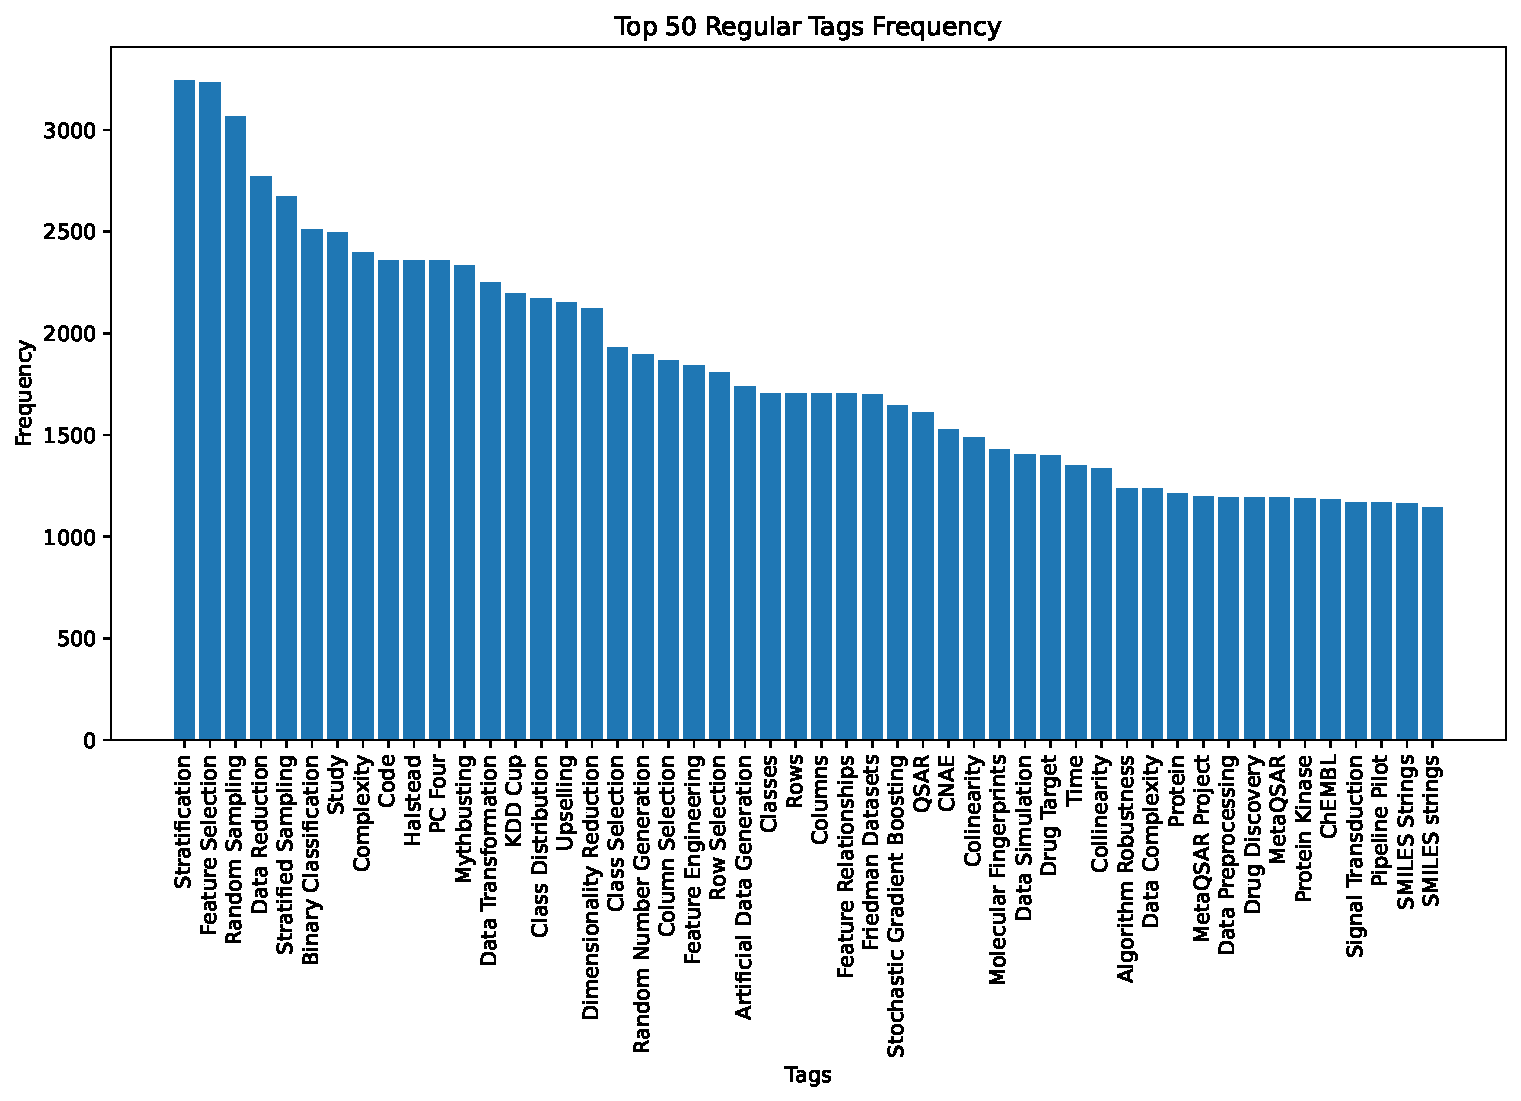
\includegraphics[width=\textwidth]{figures/top_50_frequency.pdf}
    \caption{Top 50 tags by frequency}
    \label{fig:top_50_frequency}
\end{figure}

\begin{figure}[h]
    \centering
    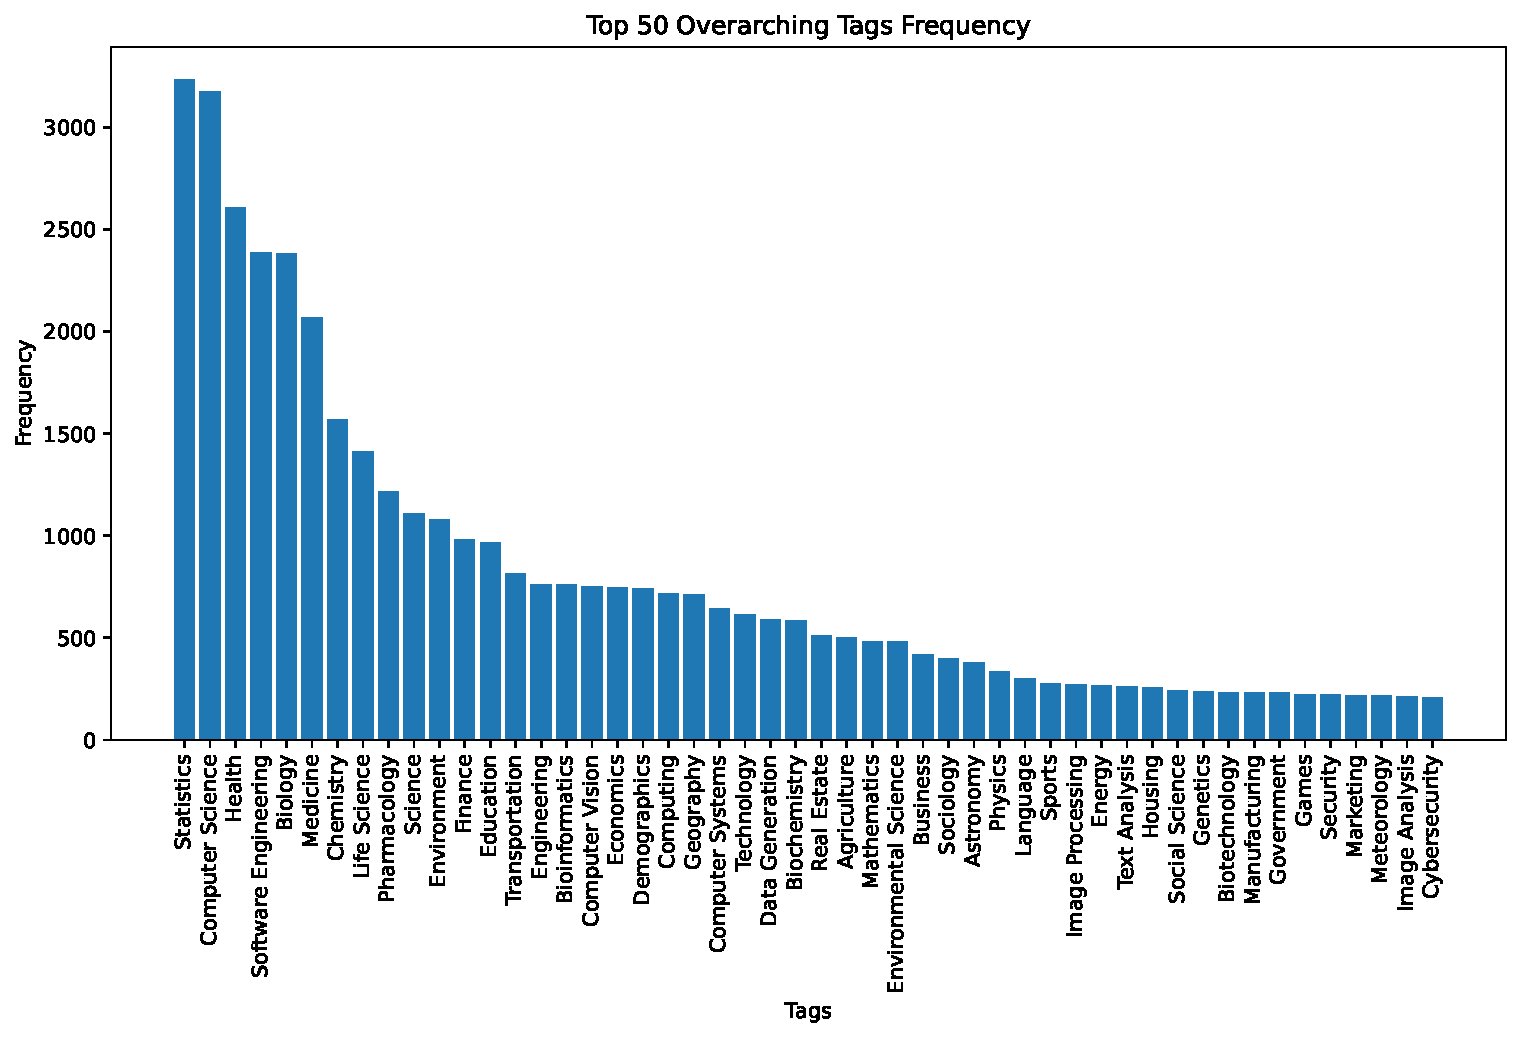
\includegraphics[width=\textwidth]{figures/top_50_overarching_frequency.pdf}
    \caption{Top 50 overarching tags by frequency}
    \label{fig:top_50_overarching_frequency}
\end{figure}

\begin{figure}[h]
    \centering
    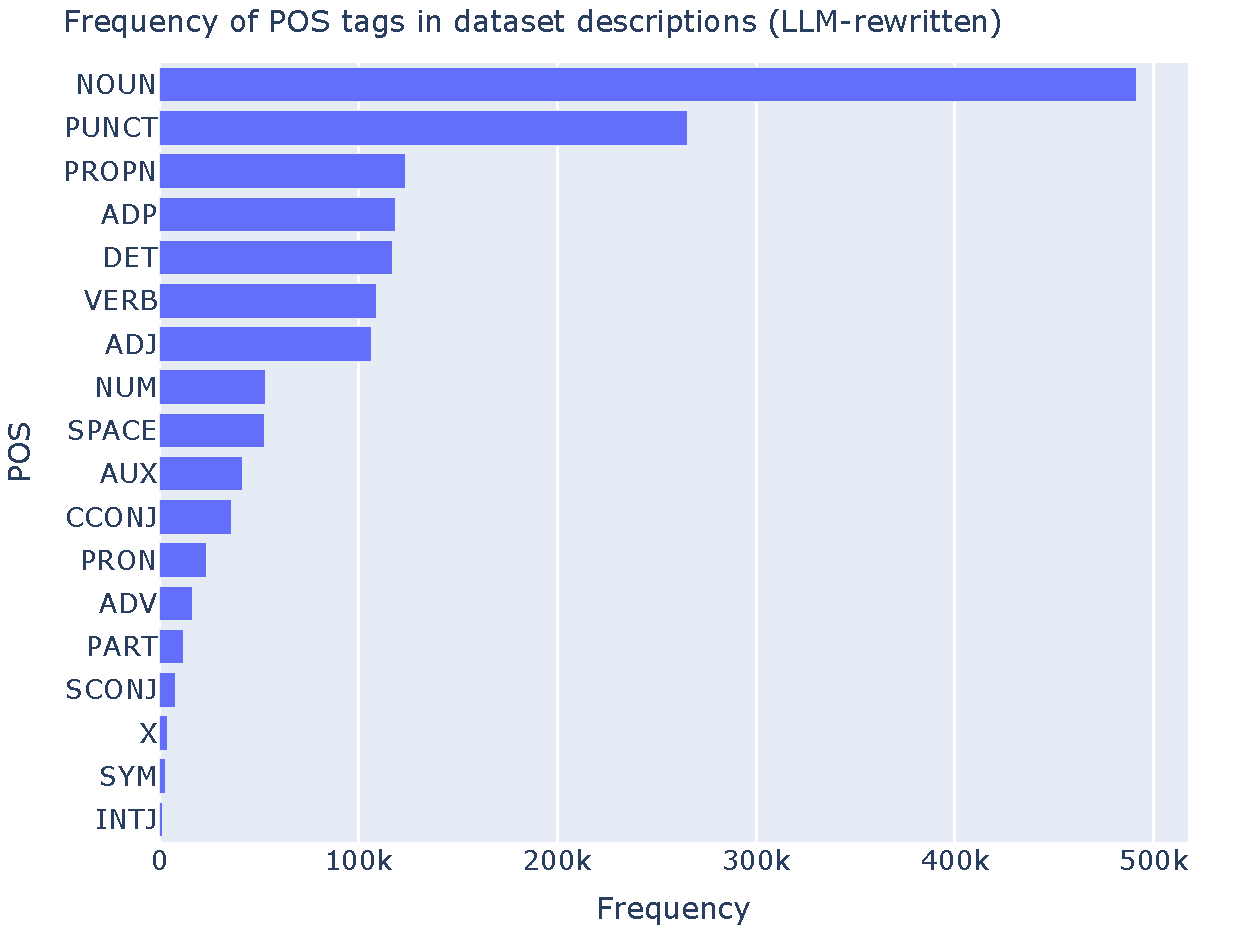
\includegraphics[width=0.8\textwidth]{figures/pos_descriptions_prompt.pdf}
    \caption{Bar chart of the most common parts of speech in dataset descriptions (LLM-rewritten)}
    \label{fig:pos_rewritten}
\end{figure}

\begin{figure}[h]
    \centering
    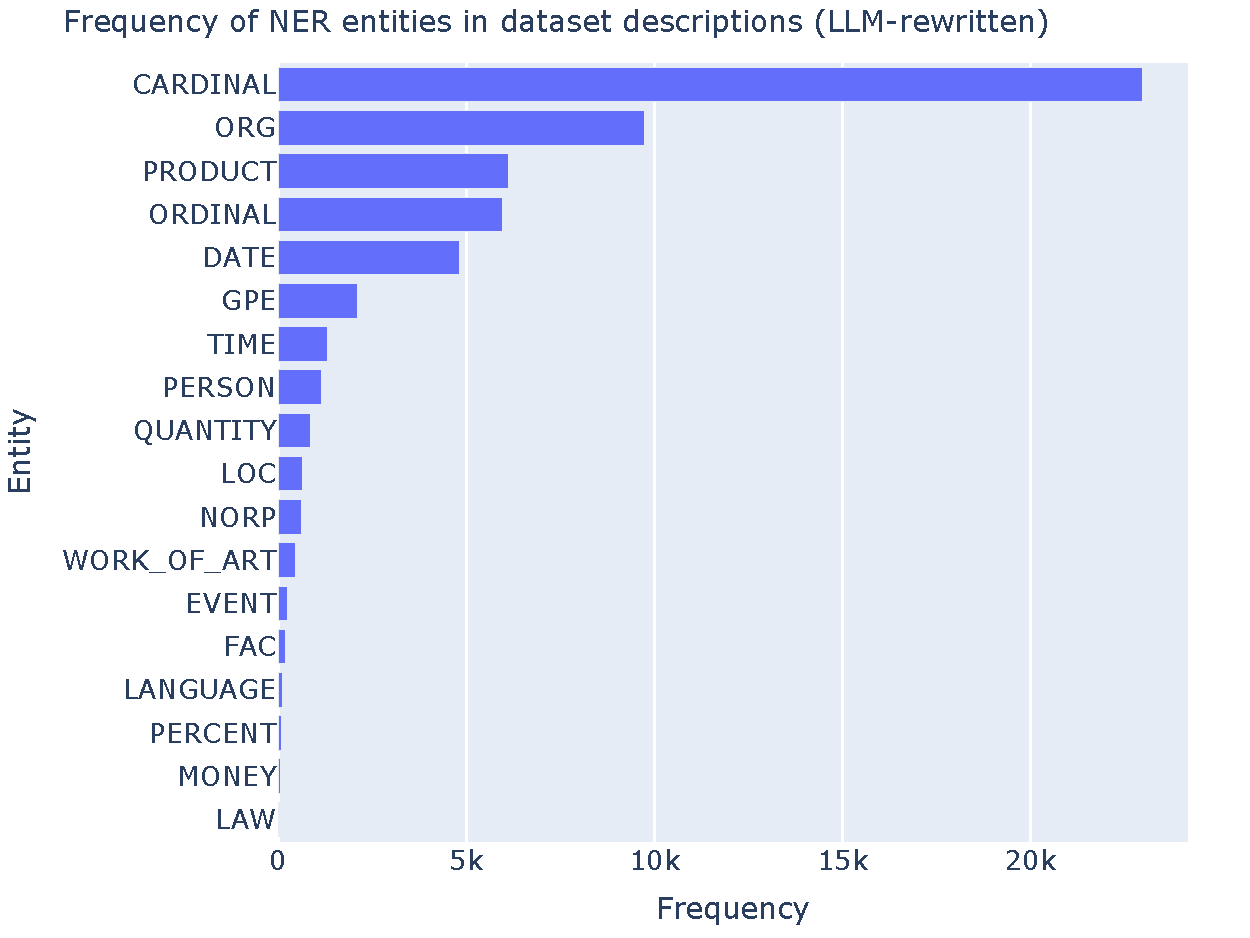
\includegraphics[width=0.8\textwidth]{figures/ner_descriptions_prompt.pdf}
    \caption{Bar chart of the most common named entities in dataset descriptions}
    \label{fig:ner_rewritten}
\end{figure}

\begin{figure}[h]
    \centering
    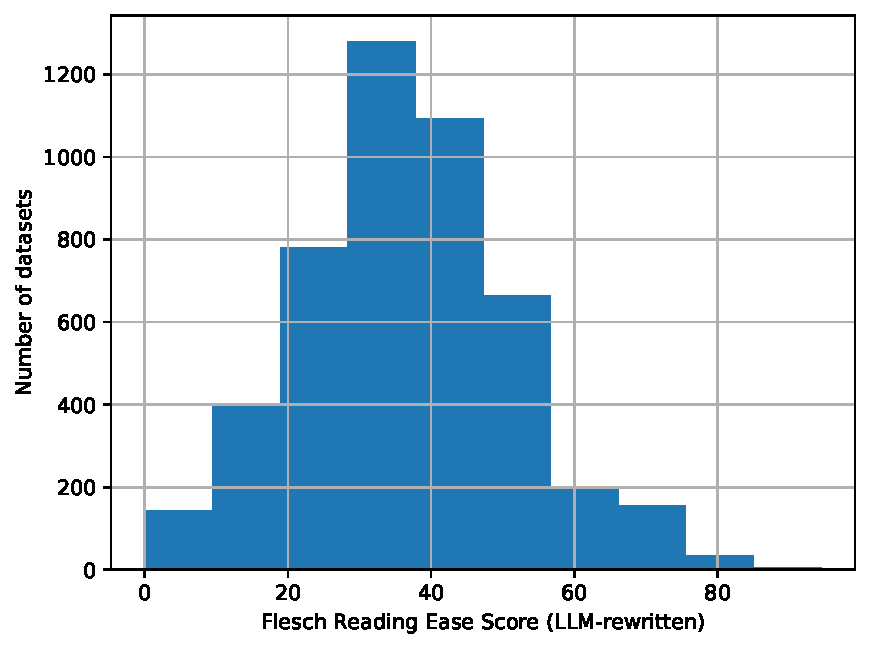
\includegraphics[width=0.8\textwidth]{figures/flesch_reading_ease_prompt.pdf}
    \caption{Histogram of the Flesch Reading Ease scores for dataset descriptions (LLM-rewritten)}
    \label{fig:flesch_reading_ease_rewritten}
\end{figure}


\begin{figure}[h]
    \centering
    \subfloat[Relevance scores]{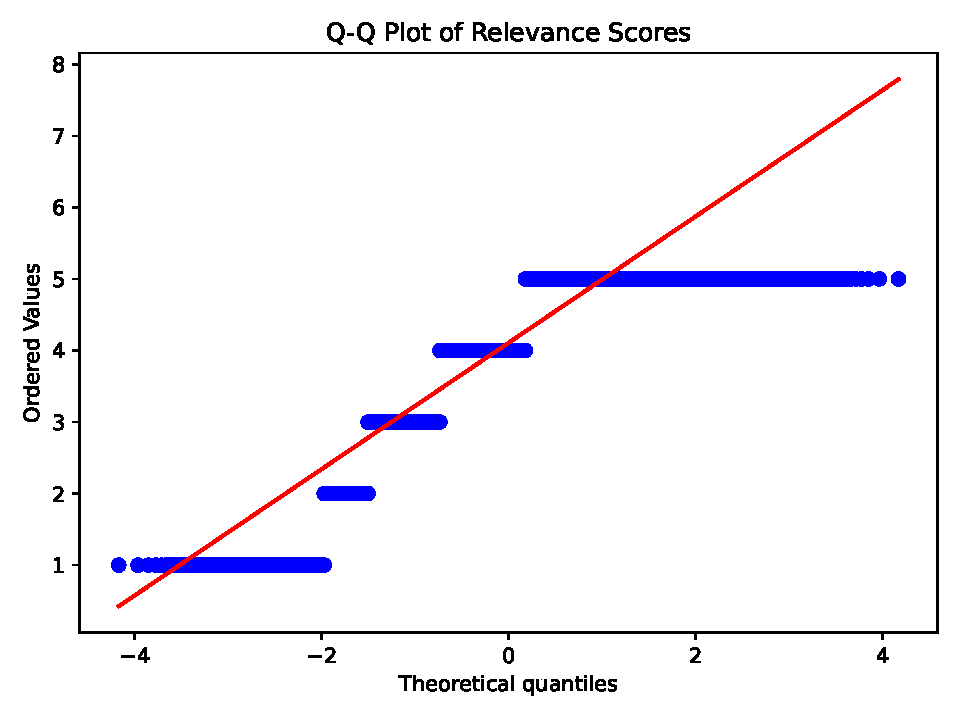
\includegraphics[width=0.5\textwidth]{figures/gpt_relevance_qq_plot.pdf}\label{fig:gpt_relevance_qq_plot}}
    \hfill
    \subfloat[Generality scores]{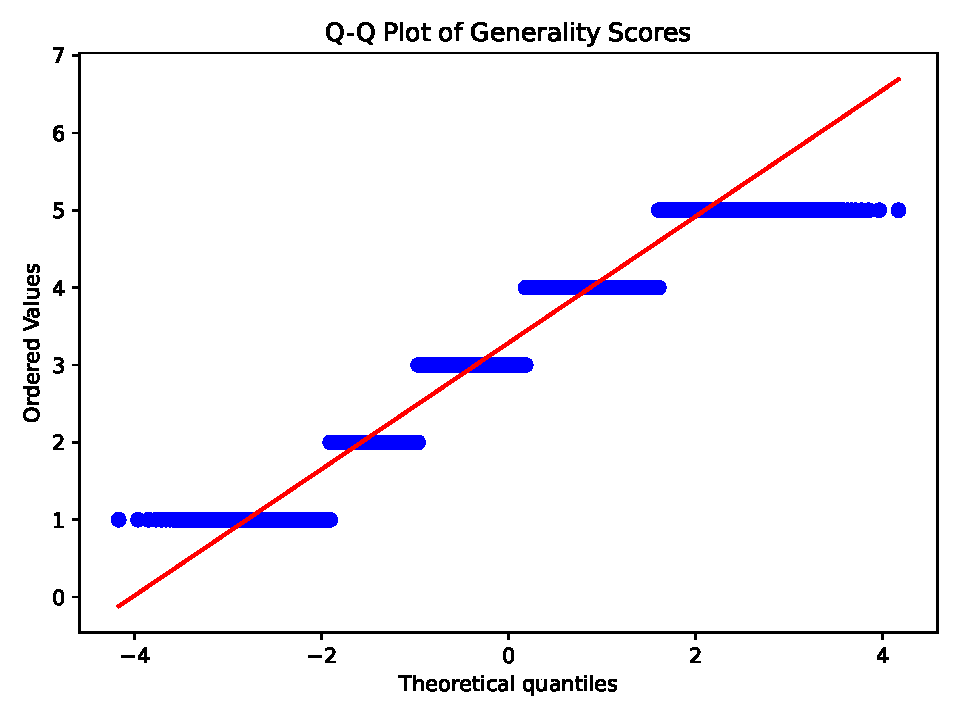
\includegraphics[width=0.5\textwidth]{figures/gpt_generality_qq_plot.pdf}\label{fig:gpt_generality_qq_plot}}

    \subfloat[Coverage scores]{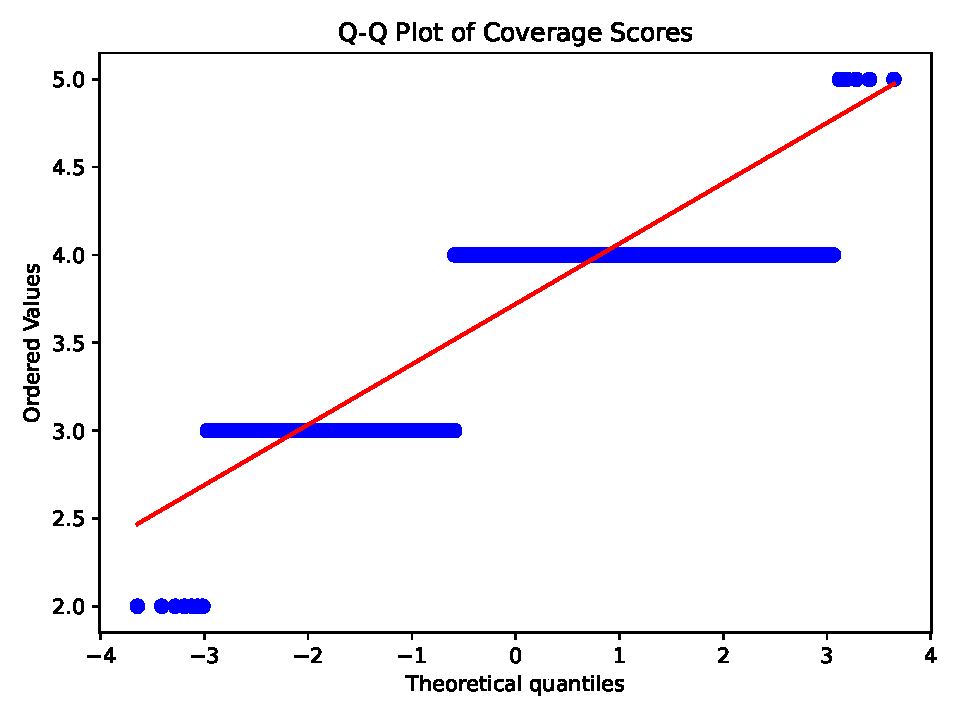
\includegraphics[width=0.5\textwidth]{figures/gpt_coverage_qq_plot.pdf}\label{fig:gpt_coverage_qq_plot}}
    \caption{Q-Q plots for evaluation metrics}
    \label{fig:all_qq_plots}
\end{figure}